% Python et ArcGIS
% Clément Delgrange
% Avril 2018

% Modules generaux
\documentclass[11pt]{article}
\usepackage[utf8]{inputenc}
\usepackage[T1]{fontenc}
\usepackage[francais]{babel} % prise en charge du francais
\usepackage[table]{xcolor} % tableaux
\usepackage{graphicx} % images
\usepackage{float}
\usepackage[font=small]{caption}

% Marges
\usepackage[left=2cm,right=2cm,top=2cm,bottom=2cm]{geometry}

% Personnalisation des titres
\usepackage{titlesec}
\titlespacing{\section}{0em}{4em}{1em}
\titlespacing{\subsection}{0em}{2em}{0em}
\titlespacing{\subsubsection}{0em}{0.5em}{0em}

% Mise en page
\setlength{\parskip}{1.2em}
\renewcommand{\floatpagefraction}{1}

% Couleurs personnalisées
\usepackage{color}
\definecolor{lightgray}{gray}{0.98}
\definecolor{gray}{rgb}{0.6, 0.6, 0.65}
\definecolor{green}{rgb}{0.133, 0.545, 0.133}
\definecolor{blue}{rgb}{0, 0, 1}
\definecolor{red}{rgb}{0.6, 0.1, 0.1}

% Liens hypertextes
\usepackage{hyperref}
\hypersetup{
	colorlinks=true,
	breaklinks=true,
	urlcolor=blue,
	linkcolor=blue,
	pdfborder=000,
	pdftex=true
}

% Mise en forme des codes python
\usepackage{listingsutf8}
\lstset{
	language=python,
	inputencoding=utf8/latin1,
	extendedchars=true,
	keywordstyle=\bfseries\ttfamily\color{blue},
	identifierstyle=\ttfamily,
	commentstyle=\color{gray},
	stringstyle=\ttfamily\color{green},
	showstringspaces=false,
	basicstyle=\footnotesize\ttfamily,
	tabsize=2,
	breaklines=true,
	extendedchars=true,
	xleftmargin=1cm,
	xrightmargin=1cm,
	backgroundcolor=\color{lightgray},
	literate=%
		{é}{{\'{e}}}1
		{è}{{\`{e}}}1
		{ê}{{\^{e}}}1
		{ë}{{\¨{e}}}1
		{û}{{\^{u}}}1
		{ù}{{\`{u}}}1
		{â}{{\^{a}}}1
		{à}{{\`{a}}}1
		{î}{{\^{i}}}1
		{ô}{{\^{o}}}1
		{ç}{{\c{c}}}1
}

% Commandes personnalisées
\newcommand{\bslash}{\code{\symbol{92}}}
\newcommand{\action}{$\Rightarrow$ }
\newcommand{\reponse}{
	\begin{tabbing}
	\hspace{2cm}\=\kill
	Réponse \> ............................................................................................ \\
 	\> ............................................................................................
	\end{tabbing}
}

\newenvironment{note}{%
	\begin{tabular}[t t]{c c}
		
\includegraphics{img/tips.png}
		 &
		\begin{minipage}[c]{0.9\linewidth}
			\begin{sffamily}
}{%
			\end{sffamily}
		\end{minipage}
	\end{tabular}
}

\newsavebox{\mybox}
\newenvironment{objectifs}{
	\begin{lrbox}{\mybox}
		\begin{minipage}{0.9\textwidth}
			\vspace{1em}
			\begin{tabular}[t t]{c c}
				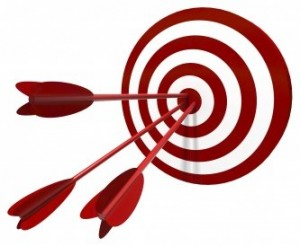
\includegraphics[width=0.1\linewidth]{img/goals.jpg} &
				\begin{minipage}[c]{0.8\linewidth}
					\hspace{2em}\textbf{\large{Objectifs :}} \\
}{
				\end{minipage}
			\end{tabular}
			\vspace{1em}
		\end{minipage}
	\end{lrbox}
	\fbox{\usebox{\mybox}}
}

\newcommand{\code}[1]{\lstinline{#1}}

\newenvironment{python}{%
	\begin{lstlisting}
}{%
	\end{lstlisting}
}


%%%%%%%%%%%%%%%%%%%%%%%%%%%%%%%%%
% Infos générales sur le document
%%%%%%%%%%%%%%%%%%%%%%%%%%%%%%%%%
\title{Python et ArcGIS}
\author{Clément Delgrange}
\date{Avril 2018}

% Entetes et pieds de page
\usepackage{fancyhdr}
\pagestyle{fancy}
\fancyhf{}
\renewcommand{\headrulewidth}{0pt}
\makeatletter
\fancyfoot[L]{\@author}
\fancyfoot[C]{-\thepage-}
\fancyfoot[R]{\@title}
\makeatother
\renewcommand{\footrulewidth}{0.5pt}


%%%%%%%%%%%%
%%% Document
%%%%%%%%%%%%
\begin{document}
\parindent=0cm


\begin{titlepage}
\makeatletter
	\begin{sffamily}
		\begin{flushleft}
			% 
\includegraphics{img/logos/ign-logo-ensg.jpg}\\[1.5cm]
		\end{flushleft}
		\begin{flushright}
			% pour mettre une image en haut à droite
		\end{flushright}

		\vspace{4cm}

		\begin{center}
			\hrule
				\vspace{1em}
				{\small \textit{Programmation SIG}}\\
				\vspace{0.5cm}
				{\huge\bfseries \@title}
				\vspace{1cm}
			\hrule

			\vspace{3.5cm}
			%\includegraphics[width=400px]{images/logo_python.png}
			\vspace{5cm}

			\large \textit{\@author}\\
			\small \textit{\@date}
		\end{center}
	\end{sffamily}
\makeatother
\end{titlepage}



\begin{objectifs}
\begin{itemize}
	\item connaître les différentes manières d'utiliser Python dans ArcMap
	\item être capable d'écrire un script de géotraitement simple
	\item connaître l'organisation générale de la bibliothèque ArcPy
\end{itemize}
\end{objectifs}


%\paragraph{Ressources utiles}
%\begin{itemize}
%	\item \textit{Cours de programmation sous SIG - Memo ArcPy}
%	\item Documentation d'ArcPy : \url{http://desktop.arcgis.com/fr/desktop/latest/analyze/arcpy}
%\end{itemize}


\section*{Préalables}
Au cours de ce TD, nous allons explorer les différentes manières d'utiliser Python avec ArcMap, l'application bureautique traditionnelle du système ArcGIS, en essayant de mettre en avant les avantages et limites de chacune des possibilités. Avant d'aborder la partie programmation, nous commencerons par un petit rappel sur l'utilisation des outils de géotraitement d'ArcMap : l'ArcToolbox et ModelBuilder.


Notre cas d'étude sera le suivant : nous disposons de données sur le positionnement des stations de métro parisiennes. Les données en question sont constituées d'un fichier csv\footnote{Comma-separated values : représentation de données tabulaires sous forme de valeurs séparées par des virgules} par ligne de métro avec les coordonnées de chaque station de la ligne. Nous souhaitons charger et mettre en forme ces données dans un SIG. Dans un autre TD, nous nous servirons des données traitées pour réaliser une application de calcul d'itinéraires.

Au cours de ce TD, nous nous contraindrons à utiliser le plus possible les outils de l'ArcToolbox. La finalité étant de programmer dans ArcMap, nous verrons en effet que l'ArcToolbox est liée à Python.

\begin{note}
ArcMap est basé sur la version 2.7 de Python, différente de celle utilisée pour les cours de Python à l'ENSG.
\end{note}



\section{Introduction aux géotraitements avec ArcMap}

\subsection{L'ArcToolbox}
\subsubsection{Découverte de l'ArcToolbox}
\action Créez un nouveau document ArcMap (\textit{TD3.mxd})

\action Dans la barre d'outils Standard, cliquez sur \textbf{ArcToolbox}.
\begin{figure}[H]
	\center 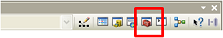
\includegraphics{img/td3/arctoolbox_bouton.png}\\
\end{figure}

ArcToolbox est une fenêtre ancrable qui peut être placée n'importe où dans l'application. Elle contient plusieurs boîtes à outils qui sont composées d'outil, de scripts et/ou de modèles. Une boîte à outils peut également être organisée en plusieurs jeux d'outils.
\begin{figure}[H]
	\center 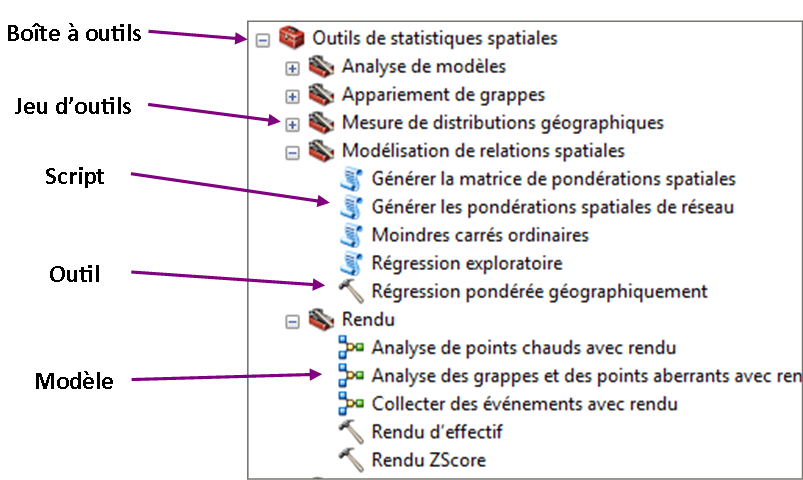
\includegraphics{img/td3/arctoolbox_composition.png}\\
\end{figure}

\action Dans la boîte à outils \textbf{Outils de conversion}, combien d'outils comporte le jeu d'outils contenant l'outil \textbf{Classe d'entités vers classe d'entités} ?

\reponse


\subsubsection{Utilisation de l'ArcToolbox pour créer une géodatabase}
Afin d'organiser les données que nous allons créer, nous souhaitons utiliser une géodatabase fichier.

\begin{note}
Esri propose deux types de géodatabase pour des utilisations bureautiques :
\begin{itemize}
	\item la géodatabase personnelle : basée sur une base Access, sa taille est limitée à 4Go (taille max d'un fichier sur un ordinateur Windows) et ne peut être utilisée par plus de 5 utilisateurs en simultané;
	\item la géodatabase fichier : utilise plusieurs fichiers pour stocker l'intégralité de la base, ce qui lui permet de ne pas être limitée à 4Go. La limite d'utilisateurs simultanés est de 20 et ses performances sont par ailleurs souvent bien meilleures.
\end{itemize}
Sauf cas exceptionnels, nous utiliserons toujours des géodatabases fichier.
\end{note}

Pour la créer, nous voudrions utiliser une Toolbox plutôt que de passer par ArcCatalog.
Il nous faut donc trouver si une telle Toolbox existe.

\action Activez l'outil de recherche en cliquant sur le bouton dans la barre d'outils \textbf{Standard}.
\begin{figure}[H]
	\center 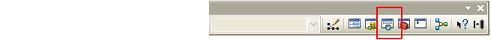
\includegraphics{img/td3/arctoolbox_bouton_recherche.png}\\
\end{figure}

\action Effectuez une recherche à l'aide des mots clé \textit{géodatabase} et \textit{créer}.

Un listing alphabétique des résultats disponibles s'affiche.

\begin{figure}[H]
	\center 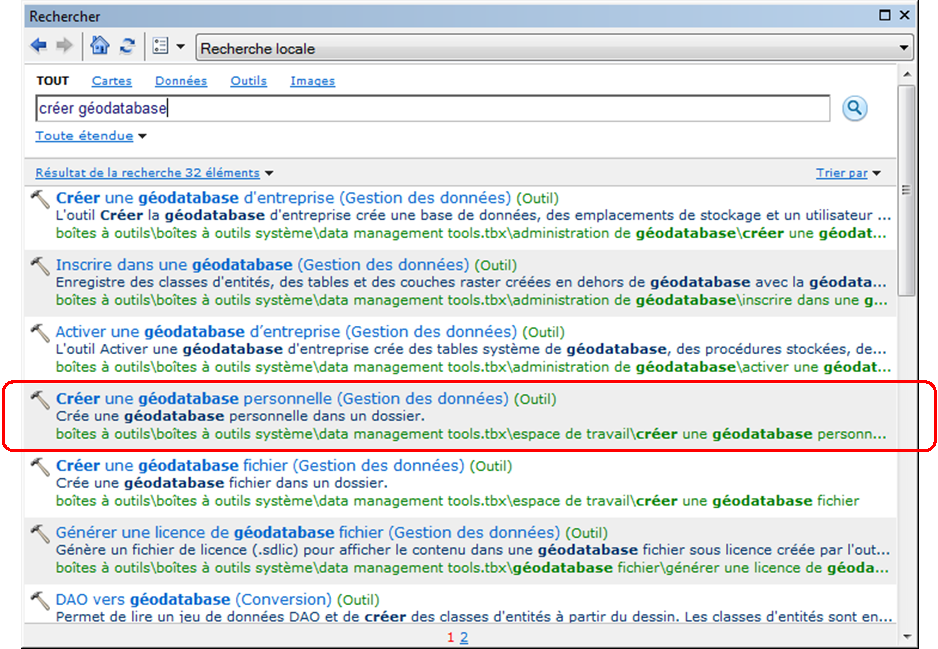
\includegraphics{img/td3/arctoolbox_recherche.png}\\
\end{figure}

Le lien en vert vous permet de localiser l'outil dans l'ArcToolbox.

\begin{figure}[H]
	\center 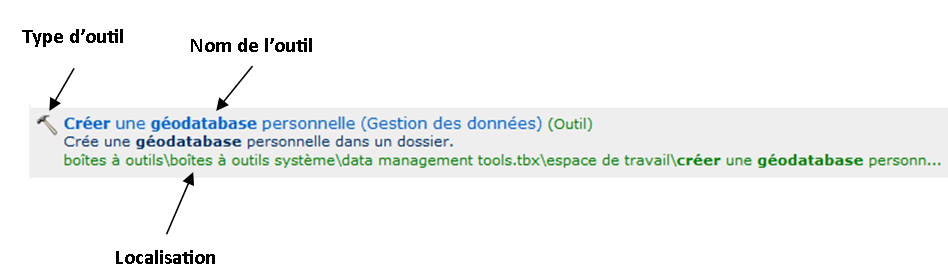
\includegraphics{img/td3/arctoolbox_recherche-2.png}\\
\end{figure}

\action Retrouvez l'outil pour créer une géodatabase dans l'ArcToolbox et exécutez-le.

\action Choisissez \textit{TD2.gdb} dans \textit{D:\textbackslash{}ProgSIG\textbackslash{}TD2}, puis cliquez sur \textbf{OK}.


\subsubsection{Définition de l'environnement de travail}
Un certain nombre de paramètres influent sur les résultats des outils de géotraitement sans pour autant être visible dans les boîtes de dialogue des outils. Il s'agit des paramètres d'environnement.

Nous pouvons par exemple spécifier un espace de travail par défaut, une étendue, un système de projection particulier pour les données en sortie de traitement, etc. Les valeurs choisies s'appliquent à tous les outils de géotraitement.

\action Dans le menu \textbf{Géotraitements}, sélectionnez l'item \textbf{Environnements...}.
\begin{figure}[H]
	\center 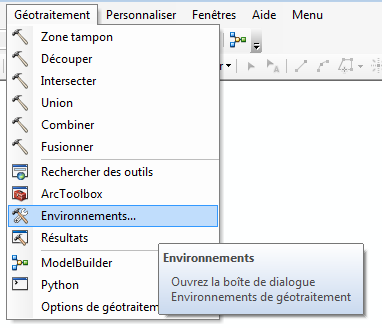
\includegraphics{img/td3/environnements_menu.png}\\
\end{figure}

\action Développez \textbf{Espace de travail} et pour \textbf{Espace de travail courant} choisissez le chemin de la géodatabase fichier que vous avez créée précédemment.
\begin{figure}[H]
	\center 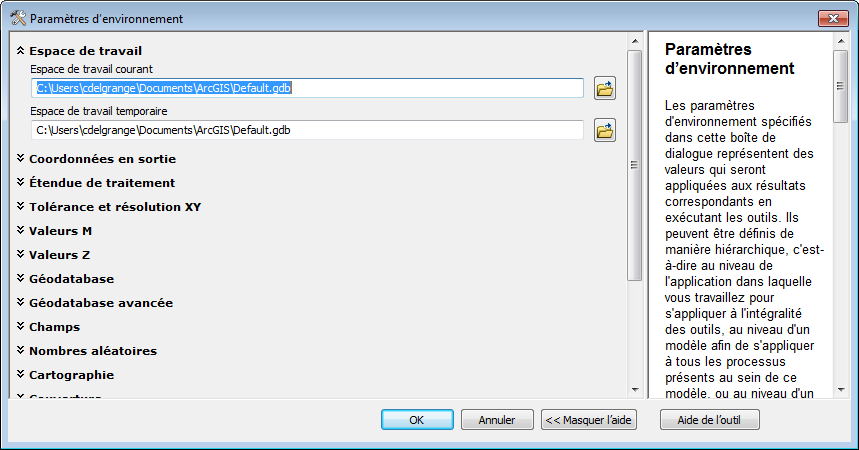
\includegraphics[width=0.8\textwidth]{img/td3/environnements_espace_travail.png}\\
\end{figure}

\begin{note}
L'espace de travail courant peut être un répertoire, une géodatabase ou un jeu de classes d'entités. Ce sera par défaut le chemin utilisé pour les données en entrée/sortie.
\end{note}

\action Pour \textbf{Espace de travail temporaire}, choisissez : \textit{D:\textbackslash{}ProgSIG\textbackslash{}TD2\textbackslash{}tmp}

L'espace de travail temporaire sera utilisé par les outils pour lesquels le chemin d'accès des données en sortie et/ou le nom de la sortie par défaut ne sera pas modifié.

Nous allons également préciser le système de coordonnées utilisé pour les données en sortie des outils.

\action Dépliez \textit{Coordonnées en sortie} et dans la liste déroulante sélectionnez \textbf{Comme spécifié ci-dessous}.

\action A la droite de la ligne qui s'active en-dessous cliquez sur le bouton représentant une main avec une feuille.

\action Recherchez et sélectionnez la projection \textit{RGF\_1993\_Lambert\_93}.
\begin{figure}[H]
	\center 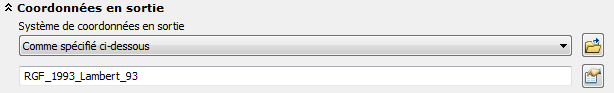
\includegraphics{img/td3/environnements_coordonnees.png}\\
\end{figure}

\action Cliquez sur \textbf{OK} pour fermer la fenêtre \textit{Paramètres d'environnement}.


\subsubsection{Utilisation de géotraitements}
Les données à notre disposition pour modéliser le réseau de métro sont constituées d'un fichier texte par ligne de métro avec les coordonnées x et y, ainsi que le nom, de chacune des stations de la ligne.

Afin de mettre en place un processus valable pour toutes les lignes, nous commençons par nous concentrer sur la ligne 1 uniquement.

\action Après avoir récupéré les données et pris connaissance du formatage des fichiers, proposez une méthodologie pour leur exploitation dans ArcMap.

\reponse

\action Dans \textbf{Outils de gestion de données > Couches et vues tabulaires}, cliquez sur \textbf{Générer une couche d'événements XY}

Cet outil crée une couche d'entités ponctuelles à partir de coordonnées X et Y définies dans une table. Le fichier fichier texte des stations fait ici office de table.

\action Configurez les champs de la manière suivante et validez.
\begin{figure}[H]
	\center 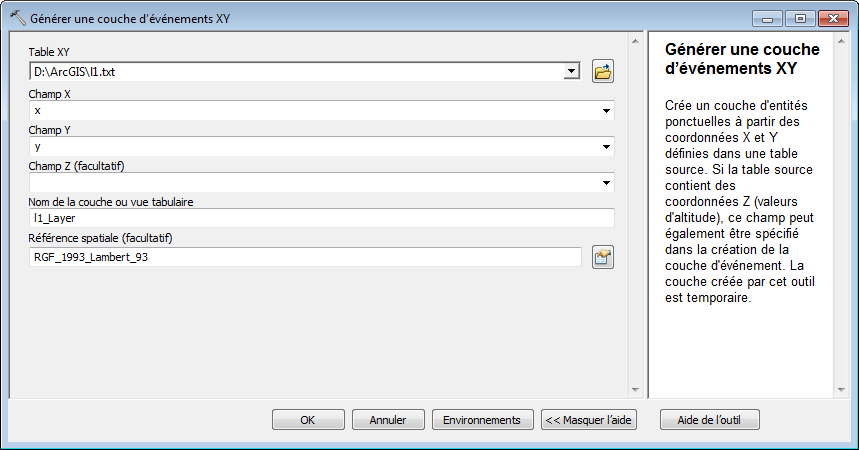
\includegraphics[width=0.8\textwidth]{img/td3/toolbox_generer_xy.png}\\
\end{figure}

Afin d'enregistrer physiquement la couche d'entités dans notre géodatabase, nous utiliserons l'outil \textbf{Classe d'entités vers classe d'entités}.

\action Retrouvez, paramétrez et utilisez cet outil pour créer la classe d'entités \textit{Stations\_ligne1} dans la géodatabase.

Pour finir, il nous reste à relier les stations de la ligne dans une polyligne.

\action Utilisez le script \textbf{Points vers lignes} pour réaliser cette opération et créer dans la géodatabase une classe d'entités \textit{Ligne1}.

A ce stade, votre document ArcMap doit contenir deux couches : les ponctuels des stations de la ligne 1 et le linéaire de la ligne.


\subsubsection{Création d'une boîte à outils personnelle}
Nous avons donc réalisé toutes les étapes de chargement des données. Sans être excessivement long, le processus serait assez longs à appliquer aux 14 lignes de métro. La première optimisation que nous allons essayer de mettre en place consistera à rassembler tous les outils utilisés dans une unique boîte à outils.

\action Effectuez un clic droit sur l'ArcTolbox > \textbf{Ajouter une boîte à outils...} :
\begin{figure}[H]
	\center 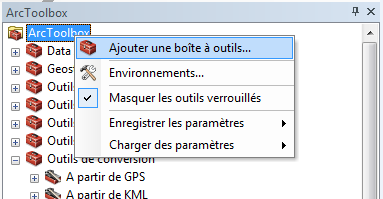
\includegraphics[width=0.45\textwidth]{img/td3/arctoolbox_ajouter.png}\\
\end{figure}

\action Dans le fenêtre qui s'ouvre, cliquez sur \textbf{Nouvelle boîte à outils} :
\begin{figure}[H]
	\center 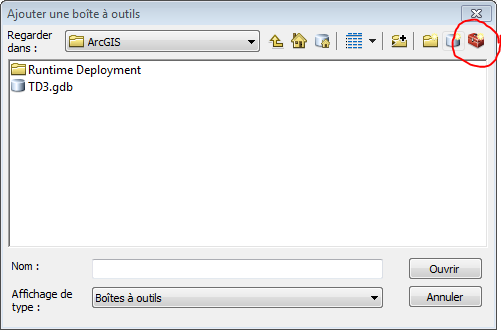
\includegraphics[width=0.45\textwidth]{img/td3/arctoolbox_ajouter-2.png}\\
\end{figure}

\action Nommez votre boîte à outils \textit{Outils\_metro.tbx}.

En validant, la nouvelle boîte à outils apparaît dans l'ArcToolbox. Il reste à y ajouter les outils. La procédure sera légèrement différent selon qu'il s'agisse d'un outil "simple", d'un script ou encore d'un modèle.

\action Clic droit sur la nouvelle boîte à outils > \textbf{Ajouter > Outil...}
\begin{figure}[H]
	\center 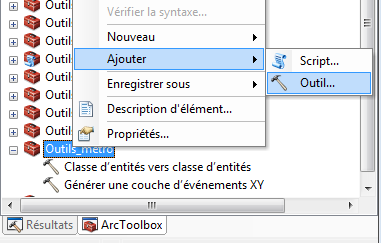
\includegraphics[width=0.45\textwidth]{img/td3/arctoolbox_ajouter-3.png}\\
\end{figure}

\action Sélectionnez les outils \textbf{Générer une couche d'événements XY} et \textbf{Classe d'entités vers classe d'entités}.

\action Clic droit sur la nouvelle boîte à outils > \textbf{Ajouter > Script...}

\action Pour le script \textit{Points vers lignes}, retrouvez le dans l'ArcToolbox et copiez-coller le dans votre boîte personnelle.

La nouvelle boîte à outils est maintenant configurée. En l'utilisant, vous pouvez ajouter à votre document les stations et lignes de la ligne 2.

\action Le résultat est-il satisfaisant? Que pourrions nous faire de mieux?

\reponse


\subsection{ModelBuilder pour enchaîner des géotraitements}
\label{modelbuilder}
\subsubsection{Créer un nouveau modèle}
ModelBuilder est un environnement permettant d'enchaîner de manière graphique des géotraitements. Nous l'utiliserons dans cette partie pour automatiser le processus de création des géométries des lignes de métro.

\action Dans ArcToolbox, faites un clic-droit sur \textit{Outils\_metro} dans la boîte à outils et cliquez sur \textbf{Nouveau > Modèle}.

\action Dans le menu \textbf{Modèle}, cliquez sur \textbf{Propriétés du modèle}.

\action Allez dans l’onglet \textbf{Général}.

\action Dans \textbf{Nom}, tapez \textit{CreationLineaireMetro}.

\begin{note}
Le nom définit comment l'outil sera appelé en programmation. Il existe certaines conventions à respecter dans le nom des modèles : pas d'espace ni de point par exemple.
\end{note}

\action Pour \textbf{Etiquette}, tapez \textit{Création d'une ligne de métro}.

\begin{note}
L'étiquette est le nom sous lequel apparaîtra votre modèle dans votre boîte à outils. Dans l'étiquette, vous pouvez utiliser les espaces et les points pour décrire de manière claire ce que fait le modèle.
\end{note}

Vous pouvez également ajouter une description plus détaillée.

\action Une fois ces champs paramétrés, cliquez sur \textbf{OK}.
\begin{figure}[H]
	\center 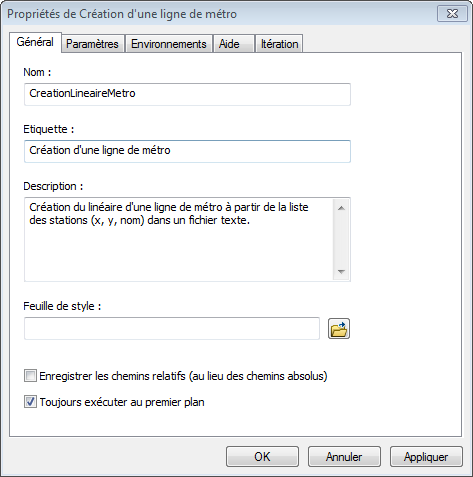
\includegraphics[width=0.55\textwidth]{img/td3/modelbuilder_creation.png}\\
\end{figure}


\subsubsection{Ajouter un outil au modèle}
\action Dans l'arborescence de l'ArcToolbox, retrouvez l'outil \textbf{Générer une couche d'événements XY} et faîtes-le glisser dans la fenêtre du modèle.

Dans un Modelbuilder, les éléments en blanc indiquent que vous avez besoin d'apporter des informations complémentaires à cet outil pour que le modèle puisse l'exécuter. Ici, il s'agit simplement de spécifier les données en entrée et d'indiquer un nom pour la couche en sortie de l'outil.

\action Dans le modèle, double-cliquez alors sur l'outil \textbf{Générer une couche d'événements XY}.

La boîte de dialogue qui apparaît est la même que celle que vous auriez obtenu si vous aviez ouvert l'outil \textbf{Générer une couche d'événements XY} depuis l'ArcToolbox.

\action Dans \textbf{Table XY}, sélectionnez pour l'instant le fichier \textit{l3.txt}.

\action Pour \textbf{Champ X} et \textbf{Champ Y} saisissez respectivement \textit{x} et \textit{y}.

\action Pour \textbf{Nom de la couche ou vue tabulaire} en sortie saisissez \textit{stations\_l3\_layer}.
\begin{figure}[H]
	\center 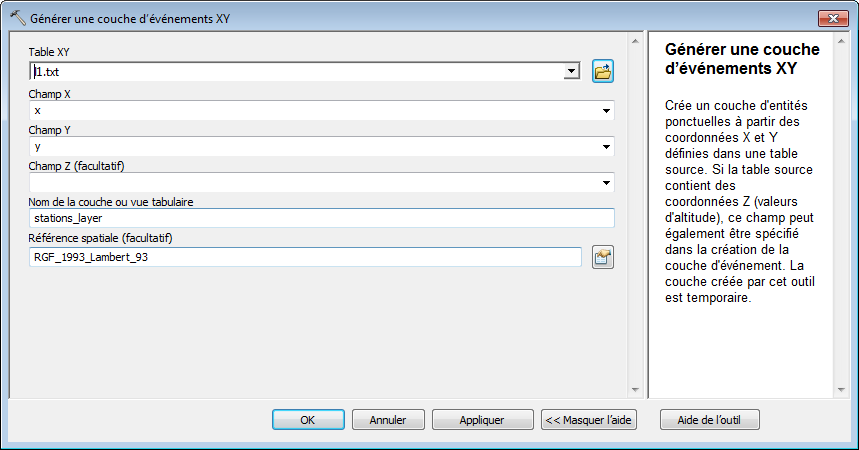
\includegraphics[width=0.8\textwidth]{img/td3/modelbuilder_creation-2.png}\\
\end{figure}

\action Validez

Dans le modèle, l'outil \textbf{Générer une couche d'événements XY} et les données en entrée/sortie sont maintenant colorés car renseignés. Il est donc prêt à être exécuté.


\subsubsection{Passer des éléments en paramètre}
La \textbf{Table XY} en entrée est en fait un paramètre du modèle : le fichier doit pouvoir être changé à chaque lancement du modèle.

\action Effectuez un clic droit sur l'élément \textit{l1.txt} du modèle > \textbf{Paramètre du modèle}.

Un petit \textit{P} apparaît en haut à droite de l'élément.
\begin{figure}[H]
	\center 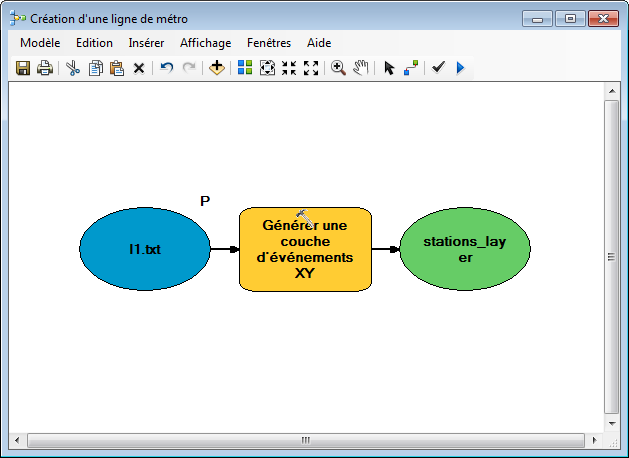
\includegraphics[width=0.45\textwidth]{img/td3/modelbuilder_creation-3.png}\\
\end{figure}

\begin{note}
Notre modèle suppose que les fichiers de départ présentent toujours la même structure, et en particulier que les champs X et Y se nomment toujours \textit{x} et \textit{y}, ce qui pourrait ne pas être le cas.

De même que pour les données, il est possible de créer des modèles génériques laissant à l'utilisateur la possibilité de saisir les valeurs des paramètres.

Pour cela, faites par exemple un clic-droit sur l’outil \textbf{Générer une couche d'événements XY}. Dans le menu contextuel, lancez le menu \textbf{Générer une variable > Paramètre de départ > Champ X}.

Un élément/paramètre (bleu ciel) vient s'intégrer au modèle.

Vous pouvez double-cliquer sur cet élément pour définir une valeur par défaut et/ou effectuer un clic-droit pour le passer en paramètre du modèle.
\begin{figure}[H]
	\center 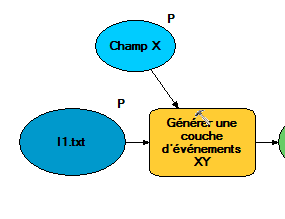
\includegraphics[width=0.3\textwidth]{img/td3/modelbuilder_creation-6.png}\\
\end{figure}

La même opération peut être effectuée pour le champ y.
\end{note}


\subsubsection{Enchaîner plusieurs outils}
\action En utilisant les mêmes méthodes, ajoutez l'outil \textbf{Classe d'entités vers classe d'entités} au modèle et paramétrez-le pour que la donnée en entrée soit la couche \textit{stations\_layer} du modèle.

\action Appelez le classe d'entités en sortie \textit{Stations\_ligne1}.

\begin{figure}[H]
	\center 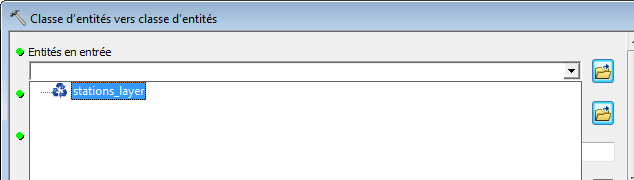
\includegraphics[width=0.6\textwidth]{img/td3/modelbuilder_creation-4.png}\\
\end{figure}

\begin{note}
La liste déroulante du modèle détecte automatiquement les données présentes dans votre modèle. Ces données sont marquées d'un icône spécifique (triangle bleu).

Un icône différent (parallélogramme jaune) apparaîtra pour dénoter les données présentes dans la table des matières d'ArcMap (si ArcMap est ouvert et que des données y sont chargées).

Bien entendu, vous pouvez aussi sélectionner des données qui ne sont ni dans votre modèle, ni dans la table des matières de votre session ArcMap.
\end{note}

\action Ajoutez enfin au modèle le script \textbf{Points vers lignes} en passant la sortie en paramètre du modèle (pour pouvoir modifier son nom).

\action Enregistrez votre modèle.
\begin{figure}[H]
	\center 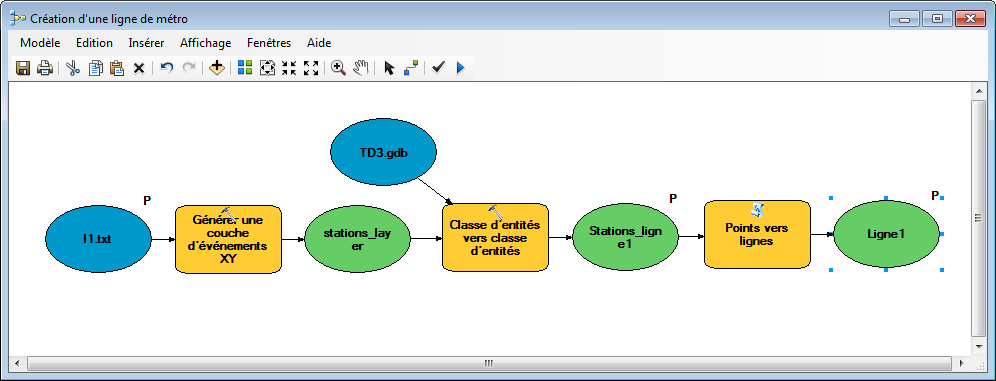
\includegraphics[width=0.7\textwidth]{img/td3/modelbuilder_creation-5.png}\\
\end{figure}

\subsubsection{Exécuter le modèle}
\action Exécutez le modèle via le menu \textbf{Modèle > Exécuter}.

\action Vérifiez que la classe d'entités \textit{Ligne3} a bien été créée.

\begin{note}
Dans le modèle, les outils ainsi que les données dérivées sont affectés d'un ombrage qui indique que les processus ont bien été exécutés. Vous devez Valider votre modèle entier (dans le menu Modèle) si vous voulez voir disparaître l'ombrage pour suivre le cheminement la prochaine fois que vous exécuterez votre modèle.
\end{note}

\action Refermez votre modèle.

\action Exécutez-le sur plusieurs lignes en double-cliquant dessus dans l'ArcToolbox et en modifiant les paramètres.

\action Le résultat est-il satisfaisant ?

\reponse



\section{Les utilisations de Python avec ArcMap}

\subsection{La console Python}
Dans ce paragraphe, nous allons nous initier à la syntaxe des commandes Python lancées depuis la console Python d'ArcMap. Nous nous servirons de ces acquis pour revenir ensuite sur notre problématique de calcul d'itinéraires dans le métro.

\action Dans la barre d'outils Standard, cliquez sur le bouton \textbf{Fenêtre Python}.
\begin{figure}[H]
	\center 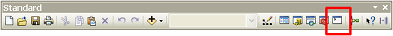
\includegraphics[width=0.6\textwidth]{img/td3/python_bouton.png}\\
\end{figure}

Vous taperez vos lignes de commandes pour accéder aux outils dans la partie de gauche. Dans la partie de droite s'affichera l'aide des commandes que vous aurez tapées.
\begin{figure}[H]
	\center 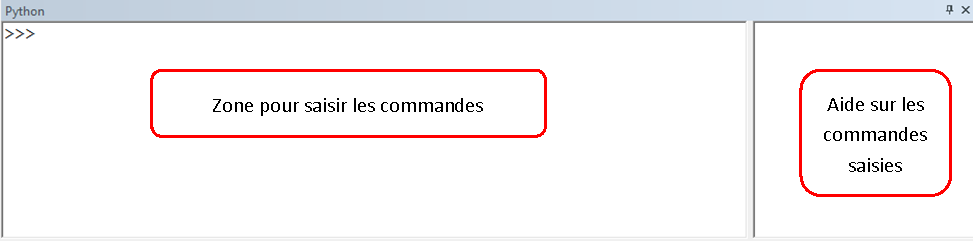
\includegraphics[width=0.7\textwidth]{img/td3/python_console.png}\\
\end{figure}

Dans un premier temps, uniquement pour nous exercer, nous allons appliquer un buffer de 20m à la ligne de métro.

\action Dans la fenêtre Python, tapez \code{arcpy.buf}

Une liste déroulante apparaît avec plusieurs commandes commençant par \textit{buf}.

\action Sélectionnez \code{Buffer\_analysis}.

\action Ouvrez une parenthèse : \code{arcpy.Buffer\_analysis(}

Un descriptif présente tous les arguments requis pour la syntaxe Buffer\_analysis dans l’aide, à droite de la fenêtre. L'argument courant est surligné en orange.
\begin{lstlisting}
Usage: Buffer_analysis (in_features , out_feature_class , buffer_distance_or_field  {line_side} , {line_end_type} , {dissolve_field...})
\end{lstlisting}

Tous les argument sont séparés par une virgule et les {} indiquent que les arguments concernés sont optionnels.

Sous la commande vous pouvez voir aussi une liste déroulante qui répertorie automatiquement toutes les classes d'entités chargées dans ArcMap et pouvant être utilisées dans la commande pour l'argument surligné.
\begin{figure}[H]
	\center 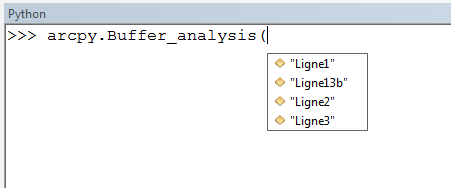
\includegraphics[width=0.45\textwidth]{img/td3/python_console_aide.png}\\
\end{figure}

\action Renseignez les arguments de la manière suivante :
\begin{itemize}
	\item \code{<In\_features>} : sélectionnez "Ligne1" dans la liste déroulante et appuyez sur \textbf{Tabulation}
	\item \code{<Out\_feature\_class>} : "Ligne1\_buff"
	\item \code{<Buffer\_distance\_or\_field>} : 50
	\item \code{{line\_side}} : "FULL" ou "" car il s'agit de la valeur par défaut
	\item \code{\{line\_end\_type\}} : "" (valeur par défaut)
	\item \code{\{dissolve\_option\}} : "ALL"
	\item \code{\{dissolve\_field;dissolve\_field...\}} : ""
\end{itemize}

Au final, la commande doit être la suivante :
\begin{lstlisting}
arcpy.Buffer_analysis("Ligne1", "Ligne1_buff", 50, "FULL", "", "ALL", "")
\end{lstlisting}

\action Appuyez sur \textbf{Entrée}.

A la fin de l'exécution de la commande, un cadre s'affiche en bas à droite de l'écran vous indiquant la réussite du traitement (ou l'échec en cas de problème).
\begin{figure}[H]
	\center 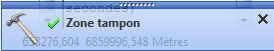
\includegraphics[width=0.45\textwidth]{img/td3/python_resultat_geotraitement.png}\\
\end{figure}

La couche \textit{Ligne1\_buff} est ajoutée au document.

Vous venez d'exécuter votre premier géotraitement avec Python. La méthode est la même pour exécuter n'importe quel autre géotraitement disponible dans ArcMap.

\action Quels peuvent être les intérêts à utiliser la console Python pour exécuter des commandes ?

\reponse

\begin{note}
ArcGIS embarque sont propre environnement Python :
\begin{lstlisting}
>>> import sys
>>> sys.path
C:\Python27\ArcGIS10.5
\end{lstlisting}
Généralement, cela ne pose pas de souci particulier, mais il conviendra tout de même d'être vigilant lors de l'installation de bibliothèque annexes (dans quelle version de Python s'installent-elles?) ou pour utiliser les outils Python d'ArcGIS en dehors d'ArcMap (version de Python utilisée?).
\end{note}


%\subsection{Exécuter un modèle depuis la console Python}
%import d'une toolbox complète et utilisation des outils de la toolbox...



\subsection{De ModelBuilder à Python}
\label{scriptautonome}
Pour dépasser les limites du modèle établit lors du paragraphe précédent, nous allons voir qu'un ModelBuilder peut s'exporter en
Nous cherchons ici à générer un script Python correspondant au ModelBuilder que nous avons réaliser précédemment pour pouvoir l'améliorer et corriger les problèmes soulevés.

\action Ouvrer la fenêtre de modification de votre modèle \textit{Création d'une ligne de métro}

\action Allez dans le menu \textbf{Modèle > Exporter > Vers un script Python...}.
\begin{figure}[H]
	\center 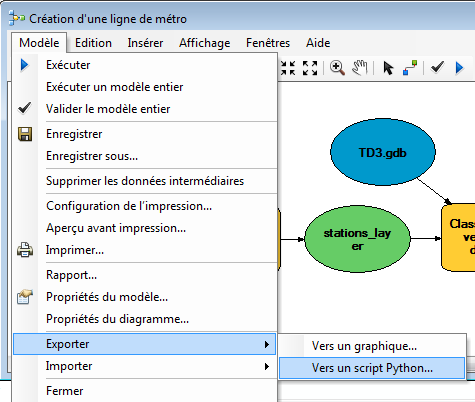
\includegraphics[width=0.6\textwidth]{img/td3/modelbuilder_export.png}\\
\end{figure}

\action Dans votre répertoire de travail, sauvegardez un fichier \textit{creation\_ligne\_metro.py}.

\action Ouvrez ce script un environnement de développement Python\footnote{PyCharm, PyScripter, Idle, Notepad++... Nous ne vous imposons pas un éditeur particulier, m}.

Nous retrouvons une structure que nous retrouverons dans les tous les scripts de géotraitement pour ArcGIS :
\begin{enumerate}
	\item Une information sur le système d'encodage utilisé (important en Python 2.7)
	\item Une en-tête décrivant le contenu du script
	\item Le chargement d'un module \code{arcpy}
	\item Des déclarations de variables
	\item Des appels de fonctions \code{arcpy} (\code{MakeXYEventLayer\_management}, \code{FeatureClassToFeatureClass\_conversion}, etc.)
\end{enumerate}

\begin{figure}[H]
	\center 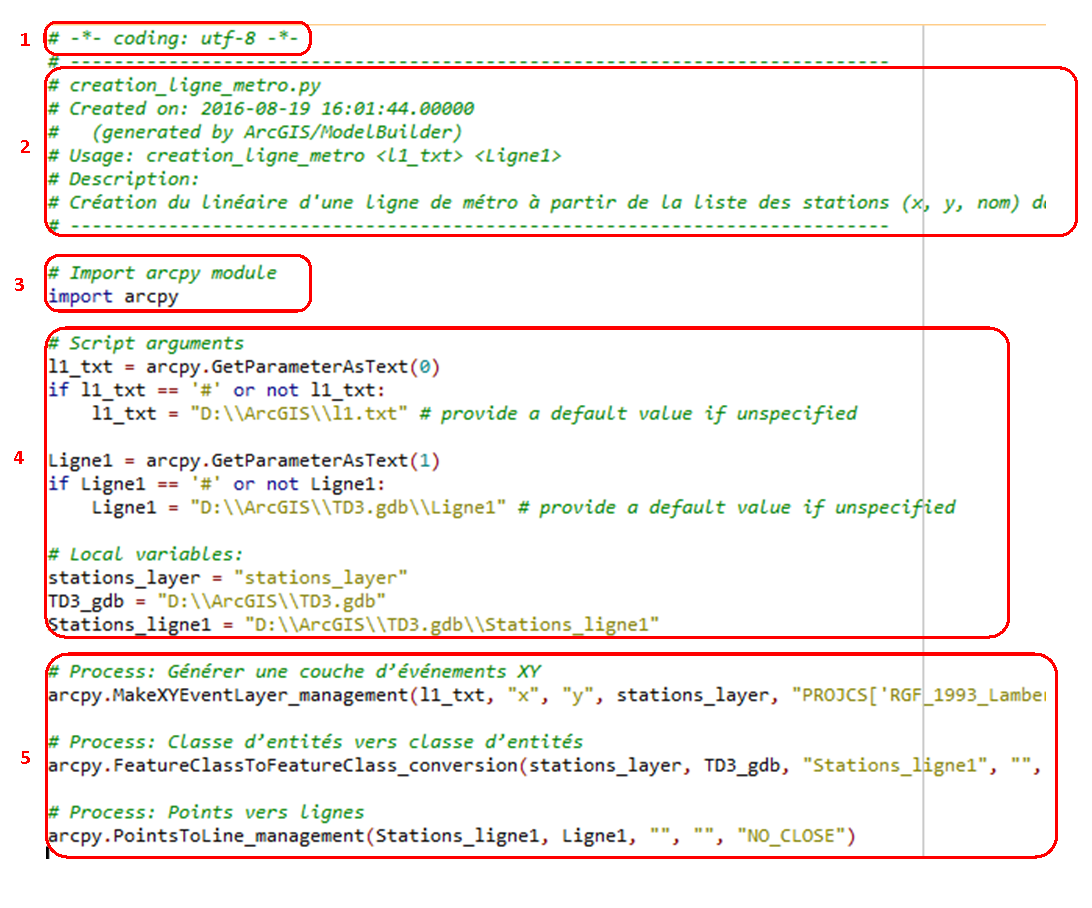
\includegraphics[width=0.8\textwidth]{img/td3/script_arcpy.png}\\
\end{figure}

\begin{note}
Dans la console Python d'ArcMap, nous n'avons pas eu besoin d'importer le module \code{arcpy} pour appeler ses fonctions.

En effet, \code{arcpy} est chargé par défaut dans la console. Partout ailleurs, il sera nécessaire de l'importer pour pouvoir l'utiliser.
\end{note}

\action	Exécutez le script.

\action Que se passe-t-il ?

\reponse

\action Essayez d'améliorer le script de sorte que le numéro de ligne et le répertoire où se trouvent les données deviennent des paramètres.

\action Lorsque le script s'exécute correctement, retournez dans ArcMap pour visualiser le résultat.

\begin{note}
Vous pouvez constater qu'il n'est pas nécessaire de conserver ArcMap ouvert pour que le script fournisse des résultats corrects.
\end{note}

Générer des scripts Python via un ModelBuilder permet généralement de faire gagner du temps pour sortir un script Python quasi fonctionnel, en réduisant la phase de recherche des fonctions ArcPy et de leur paramétrage.

Toutefois, les scripts ainsi générés sont rarement d'une propreté exemplaire. Un "nettoyage" est bien souvent nécessaire avant de pouvoir les passer en production.


\subsection{De Python à une boîte à outils}
\label{scripttoolbox}
\action Dans votre boîte à outils \textit{Outils\_metro}, ajouter le script \textit{creation\_ligne\_metro.py} (clic droit sur la boîte à outils > \textbf{Ajouter > Script...}).

Une fenêtre nous demande des informations sur le script que nous voulons ajouter.

\action Renseignez les champs de la manière suivante :
\begin{itemize}
	\item Nom : CreationLigneMetro
	\item Etiquette : Création d'une ligne de métro
\end{itemize}

\action Passez à l'étape suivante.

Il nous faut maintenant localiser le script sur le disque dur.

\action Faites pointer l'outil vers votre script \textit{creation\_ligne\_metro.py}.

\action Passez à l'étape suivante pour définir les paramètres du script :
\begin{itemize}
	\item \textit{Numéro de ligne}, de type \textit{Chaîne}
	\item \textit{Répertoire contenant les données}, de type \textit{Espace de travail}
\end{itemize}

\begin{figure}[H]
	\center 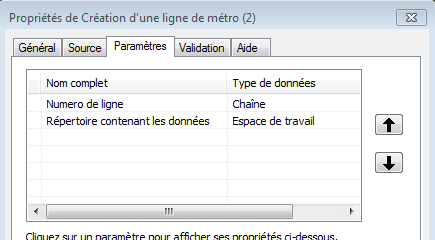
\includegraphics[width=0.55\textwidth]{img/td3/script_arcpy_param.png} \\
\end{figure}

\action Validez

\action Exécutez le script qui vient d'être ajouté à l'ArcToolbox.

A ce stade, nous avons un outil fonctionnel permettant de générer les classes d'entités pour chacune des lignes de métro. Nous avons vu que cet outil peut s'exécuter de différentes manières qui font tous appels aux mêmes fonctions d'ArcMap :
\begin{itemize}
	\item dans un ModelBuilder (voir \ref{modelbuilder})
	\item dans un script autonome (voir \ref{scriptautonome})
	\item dans un script ajouté à l'ArcToolBox (voir \ref{scripttoolbox})
\end{itemize}

Nous avons également vu que chaque Toolbox est équivalente à une fonction Python que nous savons exécuter.


\subsection{Extension Python pour ArcMap}
La dernière solution que nous allons étudier consiste à ajouter une extension dans ArcMap.
L'extension sera mieux intégrée à l'interface d'ArcMap puisqu'elle pourra prendre la forme d'un menu ou d'une barre d'outils et pourra écouter certains événements (ouverture d'une session d'édition, fermeture du document, etc.).

La diffusion des extensions est également aisée puisque nous produirons un addin ArcMap comme ceux que nous avons utilisé lors du premier TD.

\subsubsection{Création de l'extension}
Nous utiliserons un assistant pour créer la structure de notre première extension Python pour ArcMap.

\action Rendez-vous sur sur le site d'Esri\footnote{\url{https://desktop.arcgis.com/fr/arcmap/latest/analyze/python-addins/obtaining-the-python-add-in-wizard.htm}} pour télécharger l'\textit{ArcGIS Python Add-In Wizard}.

\action Décompresser l'archive.

Elle contient un exécutable qui se trouve alors dans \textit{addin\_assistant\textbackslash{}bin\textbackslash{}addin\_assistant.exe}.

\action Lancez l'assistant.

\action Pour commencer, vous devez choisir le répertoire où sera enregistré le complément (ce répertoire doit être vide).

\action Ensuite, en restant dans l'onglet \textbf{Project Settings}, indiquez quelques propriétés générales pour votre complément : nom, version, description, auteur, entreprise, etc.
\begin{figure}[H]
	\center 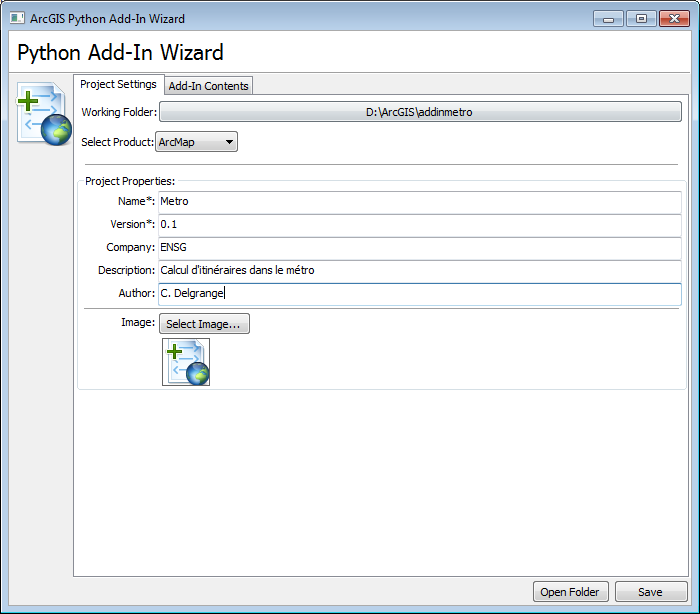
\includegraphics[width=0.55\textwidth]{img/td3/addin_assistant-1.png} \\
\end{figure}

\action Allez ensuite dans l'onglet \textbf{Add-in content}.

C'est cet onglet qui permet d'élaborer le contenu du complément.
Différents types de composants sont disponibles :
\begin{itemize}
	\item les extensions qui permettent de gérer des événements liés à l'application;
	\item les menus, et sous-menu et boutons associés;
	\item les barres d'outils et outils associés (boutons, combo box, etc.).
\end{itemize}

\action Effectuez un clic droit sur \textbf{EXTENSIONS} pour ajouter une extension.

\action Paramétrez l'extension comme sur l'image ci-dessous :
\begin{figure}[H]
	\center 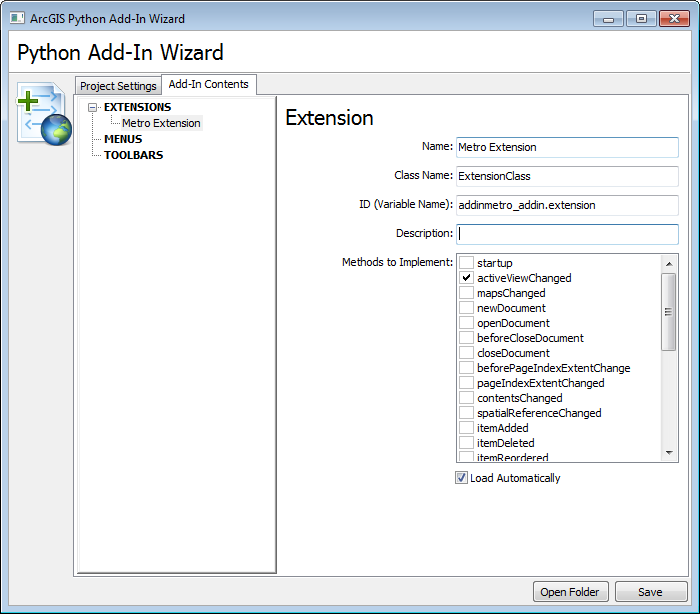
\includegraphics[width=0.6\textwidth]{img/td3/addin_assistant-2.png} \\
\end{figure}

\action De la même manière ajouter un nouveau menu que vous nommerez \textit{Métro itinéraire}.
\begin{figure}[H]
	\center 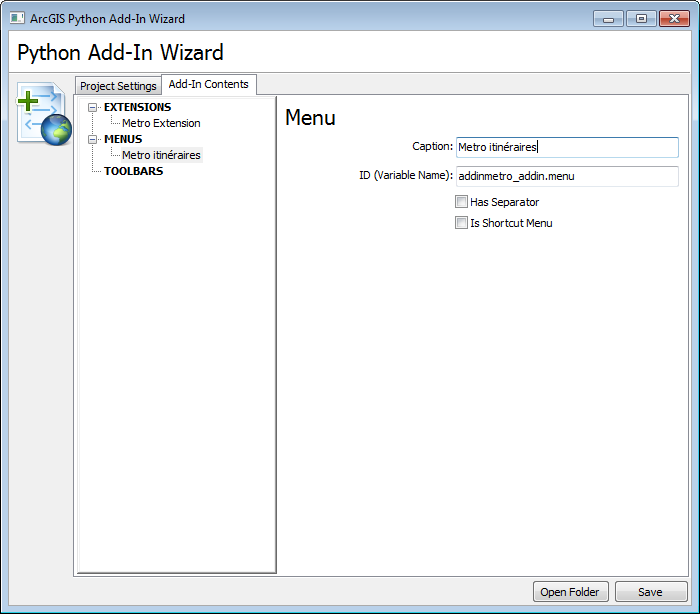
\includegraphics[width=0.6\textwidth]{img/td3/addin_assistant-3.png} \\
\end{figure}

\action Par clic droit sur votre menu \textit{Métro itinéraire}, ajoutez un bouton.

\action Configurez le bouton de la manière suivante :
\begin{figure}[H]
	\center 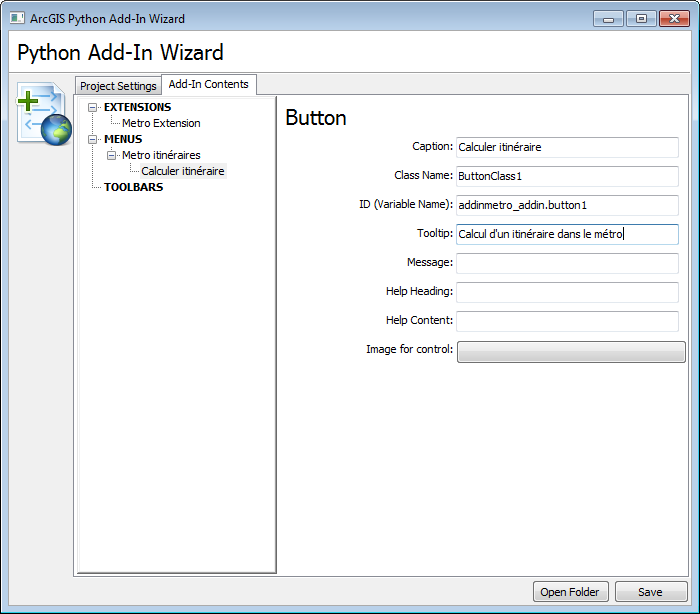
\includegraphics[width=0.6\textwidth]{img/td3/addin_assistant-4.png} \\
\end{figure}

\action Cliquez sur \textit{Save} pour enregistrer la configuration.

Vous pouvez alors refermer l'assistant et ouvrir le répertoire où vous avez enregistré votre complément.
\begin{figure}[H]
	\center 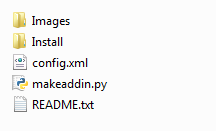
\includegraphics{img/td3/addin_repertoire.png} \\
\end{figure}

Un complément Python pour ArcMap contiendra toujours les éléments suivants :
\begin{itemize}
	\item un fichier \code{config.xml} qui contient la description de la structure de l'addin (ce que nous avons paramétré à l'aide de l'assistant);
	\item un répertoire \code{Install} contenant un fichier python (ici \code{addinmetro\_addin.py}) où se trouve la logique métier de l'addin (ie. le code qui sera exécuté lorsque l'on appuyera sur un bouton ou activera une extension);
	\item un fichier \code{makeaddin.py} permettant de générer à partir des éléments précédent un fichier \textit{.esriaddin} reconnu par ArcMap.
\end{itemize}


\subsubsection{Modification de la structure de l'extension}
Si l'assistant de création de compléments Python est très pratique pour élaborer la structure initiale d'un projet, s'en servir n'est pas obligatoire.
Dans cette partie, nous allons voir comment ajouter à un bouton à un complément existant sans passer par l'assistant : nous ajouterons un bouton d'aide au menu \textit{Métro itinéraire}.

\action Ouvrez le fichier \textit{config.xml} dans un éditeur de texte.

\action Après avoir observé le contenu des balises \code{Commands} et \code{Menus} du fichier \code{config.xml}, ajoutez un nouveau bouton au menu \textit{Métro itinéraire}

Ce bouton aura les caractéristiques suivantes :
\begin{itemize}
	\item \code{caption} = Aide
	\item \code{class} = ButtonClass2
	\item \code{id} = addinmetro\_addin.button2
\end{itemize}

L'attribut \code{class="ButtonClass2"} permet de lier le bouton à une classe Python qui sera appelé lorsque l'utilisateur cliquera sur le bouton.

\action Ouvrez le fichier \textit{addinmetro\_addin.py} pour y ajouter cette classe.

Comme pour la classe \code{ButtonClass1} déjà présente, la classe \code{ButtonClass2} doit contenir au moins deux méthodes :
\begin{itemize}
	\item le constructeur (\code{__init__()}) qui définit l'état initial du bouton;
	\item la méthode \code{onClick()} qui contient le code appelé lors d'un clic sur le bouton.
\end{itemize}

\action Créez la classe \code{ButtonClass2} avec ses deux méthodes.

Un clic sur notre bouton d'aide provoquera l'ouverture d'une fenêtre avec un message d'information à destination de l'utilisateur.
Dans un complément Python pour ArcMap, l'affichage d'une boîte de dialogue est réalisé grace à l'instruction \code{pythonaddins.MessageBox(message, titre)}.

\begin{note}
pythonaddins est un module qui apporte des fonctionnalités pour la gestion de l'interface utilisateur dans des compléments Python (il n'est utilisable que dans le cadre de compléments Python). La documentation en ligne\footnote{\url{https://desktop.arcgis.com/fr/desktop/latest/guide-books/python-addins/the-pythonaddins-module.htm}} nous renseigne sur les fonctions utilisables de ce module.
\end{note}

\action Ecrivez le code permettant d'afficher un message d'aide.

\action En exécutant le \code{makeaddin.py}, générez une première fois l'addin et installez-le pour voir s'il est conforme.


\subsubsection{Ajout de fonctionnalités}
\action Ajoutez un nouveau qui permette d'ajouter l'ensemble des stations dans une couche \textit{Stations} dans ArcMap (en vous basant sur les développement des parties précédentes).

\begin{note}
Les ArcToolbox suivantes pourront être utiles :
\begin{itemize}
	\item Supprimer les doublons
	\item Combiner
	\item Générer une couche
\end{itemize}
\end{note}

\action Complétez le code du bouton \textit{Calculer itinéraire} pour qu'il réalise les opérations suivantes :
\begin{itemize}
	\item si la couche \textit{Stations} n'est pas présente, afficher un message d'erreur;
	\item si la couche \textit{Stations} est présente, décompte du nombre de stations sélectionnées dans cette couche :
	\begin{itemize}
		\item si deux stations sont sélectionnées : lancer le calcul de l'itinéraire (nous complèterons par la suite);
		\item sinon, afficher un message d'erreur.
	\end{itemize}
\end{itemize}

\begin{note}
Pour tester l'existence d'une classe d'entités, vous utiliserez la fonction \code{arcpy.Exists(object)}.
\end{note}

\end{document}
